\documentclass[a4paper,12pt]{article}
\usepackage[utf8]{inputenc}
\usepackage[a4paper,
            bindingoffset=0.2in,
            left=1in,
            right=1in,
            top=1in,
            bottom=1in,
            footskip=.25in]{geometry}

%###############################################################################

%\input{~/layout/global_layout}


%###############################################################################

% packages begin

\usepackage[
  backend=biber,
  sortcites=true,
  style=alphabetic,
  eprint=true,
  backref=true
]{biblatex}
\addbibresource{bibliography.bib}
\usepackage[acronym]{glossaries}

\usepackage{euscript}[mathcal]
% e.g. \mathcal{A} for fancy letters in mathmode
\usepackage{amsmath,amssymb,amstext,amsthm}

\usepackage[printonlyused,withpage]{acronym}

\usepackage{mdframed}
\newmdtheoremenv[nobreak=true]{problem}{Problem}[subsection]
\newmdtheoremenv[nobreak=true]{claim}{Claim}[subsection]
\newtheorem{definition}{Definition}[subsection]
\newtheorem{lemma}{Lemma}[claim]
\newtheorem{plemma}{Lemma}[problem]

\usepackage{mathtools}
\DeclarePairedDelimiter\ceil{\lceil}{\rceil}
\DeclarePairedDelimiter\floor{\lfloor}{\rfloor}

\usepackage{enumerate}
\usepackage[pdftex]{graphicx}
\usepackage{subcaption}
% 'draft' für schnelleres rendern mitübergeben -> [pdftex, draft]
% dadruch wird nicht das bild mitgerendered, sondern nur ein kasten mit bildname -> schont ressourcen

\usepackage{hyperref}

\usepackage{tikz}
\usetikzlibrary{arrows,automata,matrix,positioning,shapes}

% for adding non-formatted text to include source-code
\usepackage{listings}
\lstset{language=Python,basicstyle=\footnotesize}
% z.B.:
% \lstinputlisting{source_filename.py}
% \lstinputlisting[lanugage=Python, firstline=37, lastline=45]{source_filename.py}
%
% oder
%
% \begin{lstlisting}[frame=single]
% CODE HERE
%\end{lstlisting}
\usepackage{algorithm}
\usepackage{algpseudocode}

\usepackage{wasysym}

\usepackage{titling}
\usepackage{titlesec}
\usepackage[nocheck]{fancyhdr}
\usepackage{lastpage}
\usepackage[absolute,overlay]{textpos}

\usepackage{kantlipsum}
\usepackage[colorinlistoftodos,prependcaption,textsize=tiny]{todonotes}

% packages end
%###############################################################################

\pretitle{% add some rules
  \begin{center}
    \LARGE\bfseries
} %, make the fonts bigger, make the title (only) bold
\posttitle{%
  \end{center}%
  %\vskip .75em plus .25em minus .25em% increase the vertical spacing a bit, make this particular glue stretchier
}
\predate{%
  \begin{center}
    \normalsize
}
\postdate{%
  \end{center}%
}

\titleformat*{\section}{\Large\bfseries}
\titleformat*{\subsection}{\large\bfseries}
\titleformat*{\subsubsection}{\normalsize\bfseries}

\titleformat*{\paragraph}{\Large\bfseries}
\titleformat*{\subparagraph}{\large\bfseries}

%###############################################################################

\pagestyle{fancy}
\fancyhf{}
% l=left, c=center, r=right; e=even_pagenumber, o=odd_pagenumber; h=header, f=footer
% example: [lh] -> left header, [lof,ref] -> fotter left when odd, right when even
%\fancyhf[lh]{}
%\fancyhf[ch]{}
%\fancyhf[rh]{}
%\fancyhf[lf]{}
\fancyhf[cf]{\footnotesize Page \thepage\ of \pageref*{LastPage}}
%\fancyhf[rf]{}
\renewcommand{\headrule}{} % removes horizontal header line

% Fotter options for first page

%\fancypagestyle{firstpagestyle}{
%  \renewcommand{\thedate}{\textmd{}} % removes horizontal header line
%  \fancyhf{}
%  \fancyhf[lh]{\ttfamily M.Sc. Computer Science\\KTH Royal Institute of Technology}
%  \fancyhf[rh]{\ttfamily Period 4\\\today}
%  \fancyfoot[C]{\footnotesize Page \thepage\ of \pageref*{LastPage}}
%  \renewcommand{\headrule}{} % removes horizontal header line
%}
%###############################################################################

\newcommand\extrafootertext[1]{%
    \bgroup
    \renewcommand\thefootnote{\fnsymbol{footnote}}%
    \renewcommand\thempfootnote{\fnsymbol{mpfootnote}}%
    \footnotetext[0]{#1}%
    \egroup
}

%###############################################################################

\title{
  \vspace{6cm}
  \normalsize{DD2365 VT25 Advanced}\\
  \normalsize{Computation in Fluid Mechanics}\\
  \Large{On Simulating the}\\
  \Large{Kelvin Helmholtz Instabilities}
}
\author{
  \small Paul Mayer\\[-0.75ex]
%  \footnotesize\texttt{MN: }\\[-1ex]
  \scriptsize\texttt{pmayer@kth.se}
}
\date{}

%###############################################################################
% define Commands

\newcommand{\N}{\mathbb{N}}
\newcommand{\R}{\mathbb{R}}
\newcommand{\Z}{\mathbb{Z}}
\newcommand{\I}{\mathbb{I}}

\newcommand{\E}{\mathbb{E}}
\newcommand{\Prob}{\mathbb{P}}

\renewcommand{\epsilon}{\varepsilon}

%###############################################################################
\makeatletter
\renewcommand*{\@fnsymbol}[1]{\ensuremath{\ifcase#1\or \dagger\or \ddagger\or
   \mathsection\or \mathparagraph\or \|\or **\or \dagger\dagger
   \or \ddagger\ddagger \else\@ctrerr\fi}}
\makeatother
%###############################################################################

\begin{document}

\begin{textblock*}{\paperwidth}(0cm,2.25cm)
    \centering 
    
\includegraphics[width=3.75cm]{assets/kthlogo.png}
\end{textblock*}

\maketitle
%\thispagestyle{firstpagestyle}
% content begin
%

\section*{Abstract}
Kelvin–Helmholtz instabilities emerge in shear layers between fluid regions of differing velocities and are key phenomena in both natural and industrial fluid dynamics. This project investigates the influence of grid resolution and Reynolds number on the development and persistence of Kelvin–Helmholtz instabilities using the incompressible Navier–Stokes equations. A Galerkin Finite Element Method framework implemented in FEniCS is used to simulate 2D shear flows with perturbed initial conditions.
The study explores how numerical resolution and viscous dissipation affect the onset and evolution of rotational structures by tracking the rotational component of the velocity gradient via Triple Decomposition.
Simulations show that insufficient grid resolution suppresses instability formation, while lower Reynolds numbers lead to rapid vortex dissipation due to enhanced viscous effects.
A grid resolution of at least 32 and Reynolds numbers above 1000 are required for meaningful vortex evolution within the simulation time frame.
While the project is primarily exploratory and did not use validated benchmarks, it provides a foundational learning experience in computational fluid dynamics and fluid instability modelling.
\newpage

\tableofcontents

\section*{Acronyms}
\begin{acronym}
 \acro{K-H}{Kelvin-Helmholtz}
 \acro{FEM}{Finite Element Method}
 \acro{TDC}{Triple Decomposition}
 \acro{CFD}{Computational Fluid Dynamics}
\end{acronym}
\newpage

\section{Introduction}
\ac{K-H} instabilities are instabilities that form in the shear boundary between two fluids with different velocities \cite{Helmholtz1868}.
This phenomena has been studied in the real world as well as in experiments \cite{DeSilva1996}. 

In this project, I investigated how the grid resolution and Reynolds number influences the accuracy and dynamics of \ac{K-H} instability simulations using the incompressible Navier–Stokes equations.
The numerical framework is based on the Galerkin finite element method (FEM) implemented in the FEniCS library, a open-source platform for solving partial differential equations.
Since the \ac{K-H} instability is characterized by the exponential growth of small-scale perturbations, accurately resolving these features requires sufficient numerical resolution --— particularly close to high velocity gradients.

This study focuses on the onset time of the instability.
I compare the magnitude over the rotational dimension of the velocity field to quantify differences between simulations and try to identify a minimum resolution required to obtain meaningful results.
Additionally, I want to observe if the behaviour of the instabilities changes when working with different Reynolds numbers.

I intent this project to be an introduction for me to the world of simulating fluids.
The initial conditions for the simulations are taken from \href{https://levelup.gitconnected.com/create-your-own-finite-volume-fluid-simulation-with-python-8f9eab0b8305}{this blogpost}, which presents a python implementation we optimised in a different project.
A personal goal of mine is to replicate somewhat similar vortex structures using a different (finite element) simulation approach.

\section{Methodology}
\subsection{Galerkin Finite Element Method}
For this project I used FEniCS, which is a Galerkin \ac{FEM} Framework.
The Galerkin \ac{FEM} Method is defined as: find a trial function $U \in V_h$, such that
\begin{equation}
  \label{eq:galerkinfem}
  \int_0^1 U'(x) v'(x) dx = \int_0^1 f(x) v(x) dx,
\end{equation}
for all test functions $v \in V_h$.
We use piecewise linear basis functions as our test functions.

\subsection{The governing equations}
For the simulation I used the incompressible Navier-Stokes equations which take the form
\begin{align}
  \frac{\partial u}{\partial t} + (u\cdot \nabla)u - \nu \Delta u + \frac{1}{\rho} \nabla p - \frac{1}{\rho} f &= 0,\\
  \nabla \cdot u = \frac{\partial u_x}{\partial x} + \frac{\partial u_y}{\partial y}  &= 0.
\end{align}

To simulate the instability, the force term will be 0.
To generate a shear-layer where the instability can develop, we need appropriate initial conditions.
I chose a high velocity jet-stream moving to the right against a background stream moving to the left.
To help the instabilities to start forming, we add a small perturbation $\psi$ to the $y$-Component of the velocity:

\begin{equation}
u_0 = \begin{pmatrix}-1 + 2 * (\text{abs}(x[1] - 0.5) <= 0.5)\\
        \psi(x,y)\end{pmatrix}\,
\end{equation}
\begin{equation}
        p_0 = 2.5,
\end{equation}
and
\begin{align*}
  \psi(x,y) = 0.1 * \sin(4 * \pi * x[0]) * \Bigg(&\exp\left(-\left(\left(x[1] - \frac{1}{4}\right) * \left(x[1] - \frac{1}{4}\right)\right) / \left(2 * \sigma^2\right)\right) \\
  &+ \exp\left(-\left(\left(x[1] - \frac{3}{4}\right) *\left(x[1] - \frac{3}{4}\right)\right) / \left(2 * \sigma^2\right)\right)\Bigg),
\end{align*}
where $\displaystyle \sigma = \frac{0.05}{\sqrt{2.0}}$.

\subsection{Rotation onset}
There are multiple approaches to quantify the rotational magnitude of a velocity field.
One idea is to compute the vorticity (or curl) for the velocity field and integrate over the domain. In 2D this is given as:
\begin{equation}
  \label{eq:curl}
  \int_{\Omega} \nabla \times v\ dx = \left(\frac{\partial u_y}{\partial x} - \frac{\partial u_x}{\partial y}\right)
\end{equation}

However, the vorticity is not a useful tool for measuring the onset of the stability, because it can also capture the shear stress in a point.
Because we initialise the simulation with a high shear force, the actual rotational force is smaller than the shear stress in the beginning, making this an inappropriate tool for measuring the onset of the instability.

A better approach is to use the \ac{TDC} of the velocity gradient tensor \cite{Hoffman2021a, Keylock2018}.
We calculate
\begin{align}
  \label{eq:tripledec}
  \int_{\Omega} u_{\textrm{RR}} dx &= \int_{\Omega} (Q^{T} (\nabla u)_{\textrm{RR}} Q) (x_0)(x - x_0) dx
\end{align}
To quantify and compare the different runs, we measure this for $t \in [0.1, 0.2, ..., 5]$.

\subsection{Implementation}
I simulated the Instability using FEniCS \cite{Alnaes2015} on Google Colab \cite{Colab2025} with the help of \cite{FEMColab2021}.
The simulation is based on the Navier-Stokes template (found \href{https://github.com/johanhoffman/DD2365_VT25/blob/main/template-report-Navier-Stokes.ipynb}{here}) provided in the course.
It uses a residual based stabilisation and piecewise linear test functions to solve for the velocity and pressure fields.

The periodic boundary conditions for the velocity field are implemented using a mapping.
\begin{lstlisting}
class PeriodicBoundary(SubDomain):
    # Left boundary is "target domain" G
    def inside(self, x, on_boundary):
        return bool(x[0] < DOLFIN_EPS and x[0] > -DOLFIN_EPS and on_boundary)

    # Map right boundary (H) to left boundary (G)
    def map(self, x, y):
        y[0] = x[0] - L
        y[1] = x[1]

[...]

V = VectorFunctionSpace(mesh, "Lagrange", 1, constrained_domain=PeriodicBoundary())
Q = FunctionSpace(mesh, "Lagrange", 1, constrained_domain=PeriodicBoundary())
\end{lstlisting}
For the pressure I used only Neumann-boundary conditions.
Because only the pressure gradient is defined, I added a small mass matrix to the momentum equation to make the equation well defined.

\subsection{Experiment Setup}
The domain is 2D and quadratic. 
I ran the simulation for varied Reynolds numbers (and fixed grid resolution) as well as varied grid resolutions (for a fixed Reynolds number).
I plotted the magnitude of the rotational part of the velocity gradient's \ac{TDC}.
For visualisation purposes I computed the curl of the velocity field.
The plotting is performed for 50 equidistant time steps and runs from $t=0$ till $t=T=5$.

\newpage
\section{Results}
We ran the simulations for varying grid sizes and Reynolds numbers.
As a reference simulation, we choose a Reynolds number of 10000 and a grid resolution of 64.

A visualisation of the reference simulation can be found \href{https://github.com/paulmyr/DD2365-AdvancedCFD/blob/master/project/presentation/vid/velocity_lic_64.avi}{here}.

\subsection{Sensitivity to grid}
\label{sec:result_grid}

\begin{figure}
     \centering
     \begin{subfigure}[b]{0.45\textwidth}
         \centering
         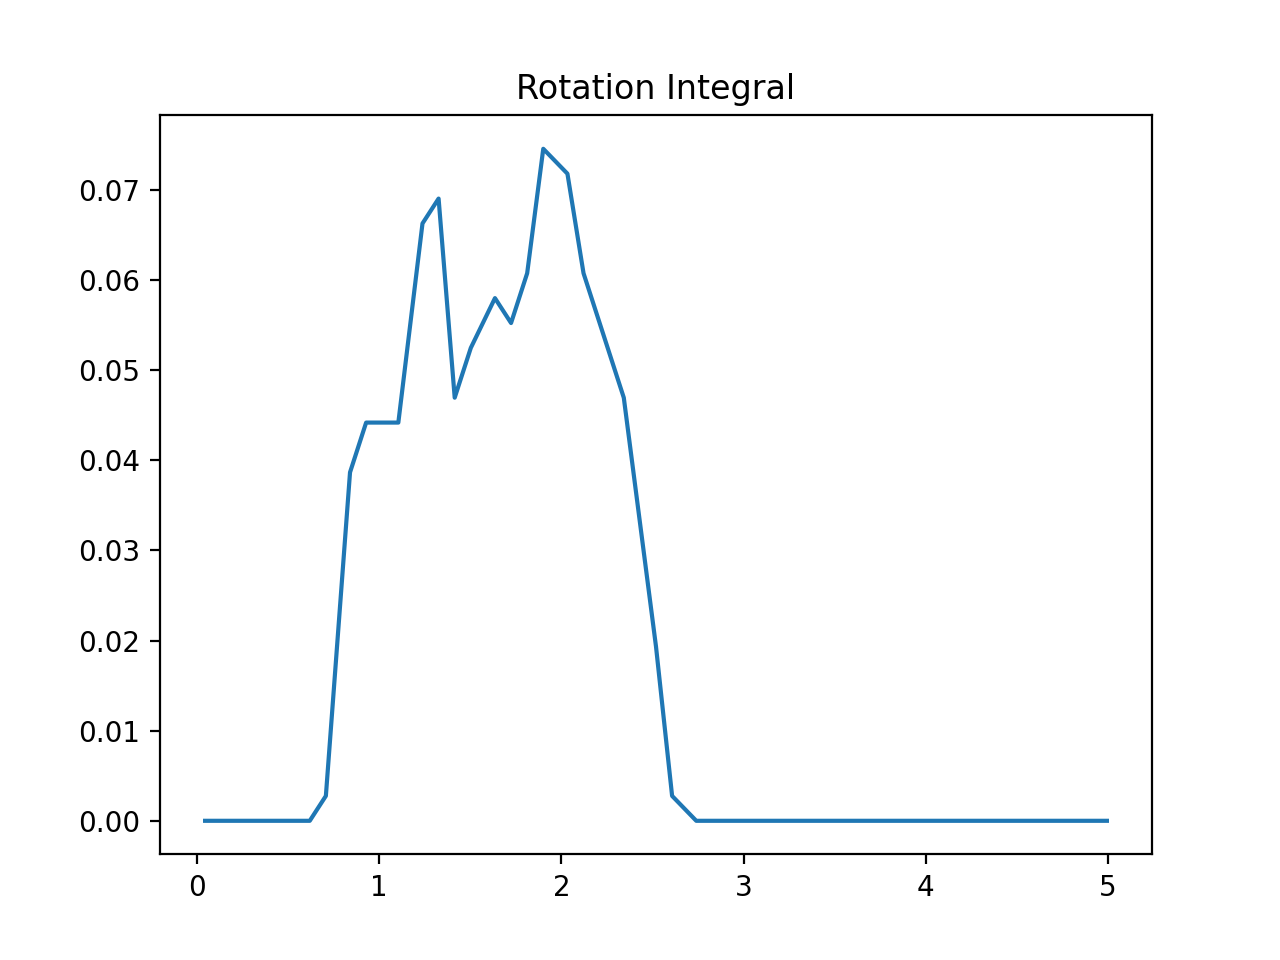
\includegraphics[width=\textwidth]{imgs/results-KHI-RE10000.0-RSL16-rr_integral}
         \caption{resolution: 16}
         \label{fig:re10000-rs16}
     \end{subfigure}
     \hfill
     \begin{subfigure}[b]{0.45\textwidth}
         \centering
         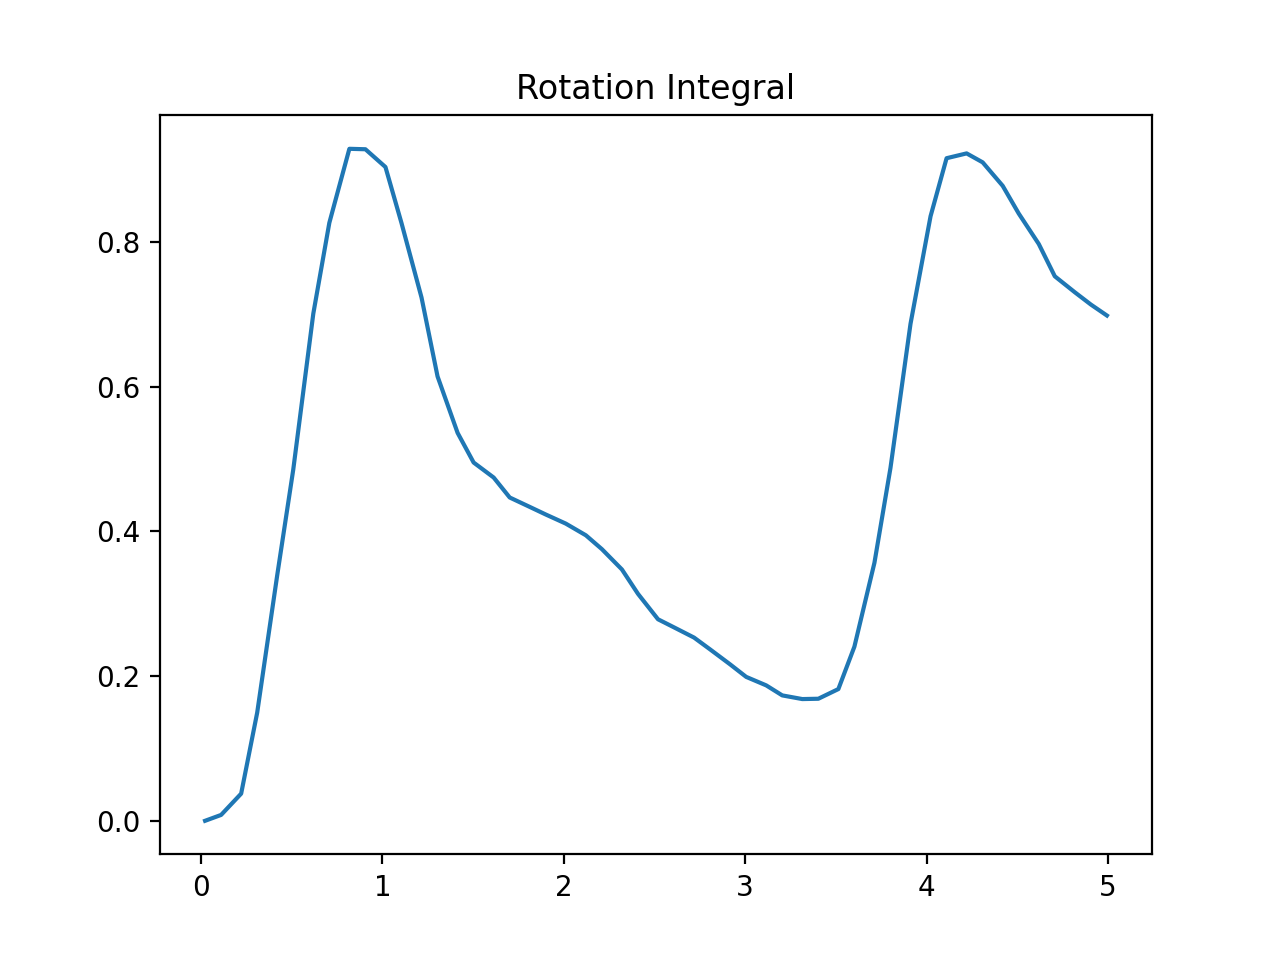
\includegraphics[width=\textwidth]{imgs/results-KHI-RE10000.0-RSL32-rr_integral}
         \caption{resolution: 32}
         \label{fig:re10000-rs32}
     \end{subfigure}
     \hfill
     \begin{subfigure}[b]{0.45\textwidth}
         \centering
         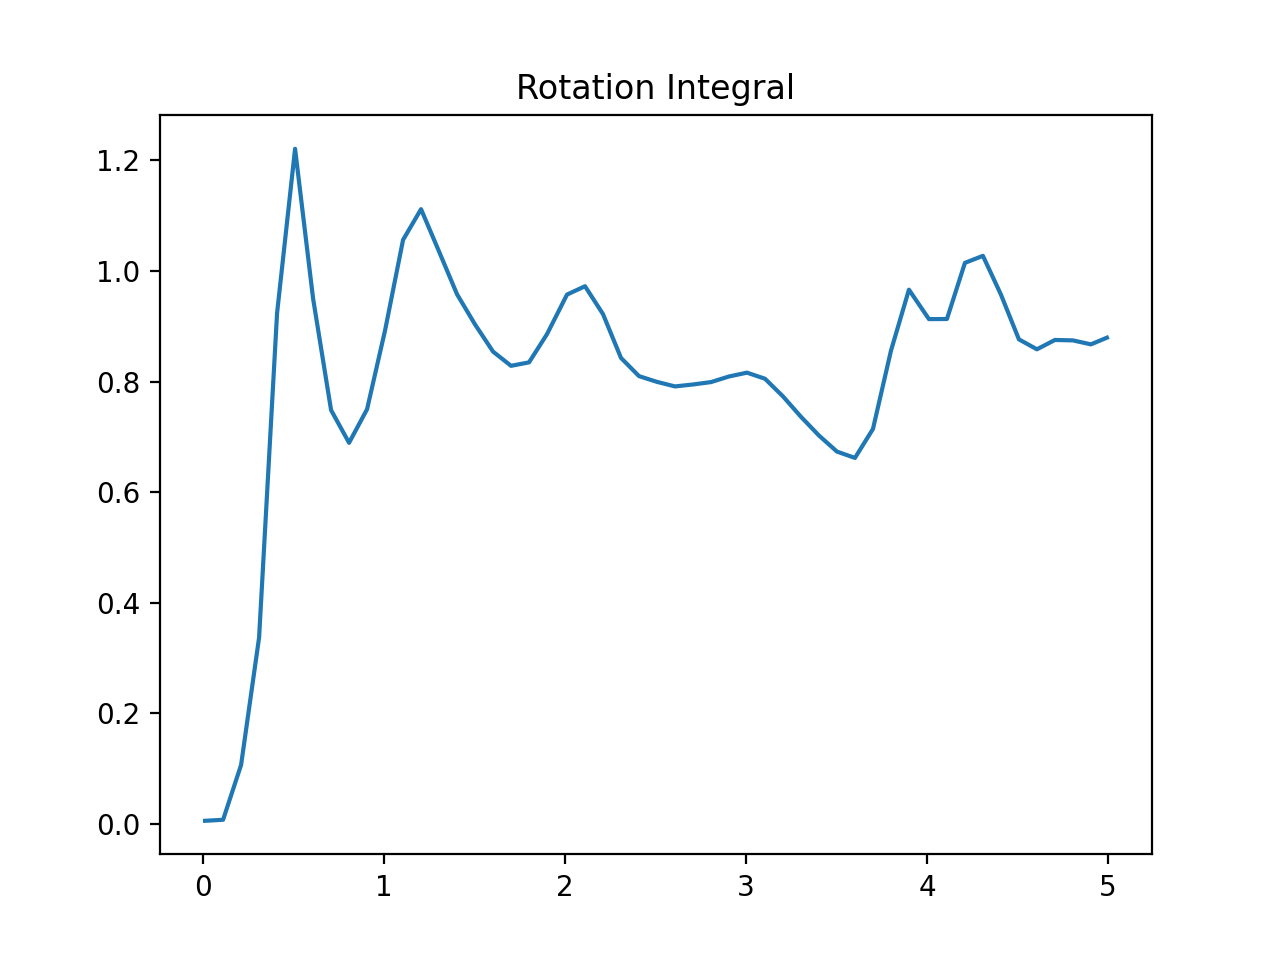
\includegraphics[width=\textwidth]{imgs/results-KHI-RE10000.0-RSL64-rr_integral}
         \caption{resolution: 64}
         \label{fig:re10000-rs64}
     \end{subfigure}
     \hfill
     \begin{subfigure}[b]{0.45\textwidth}
         \centering
         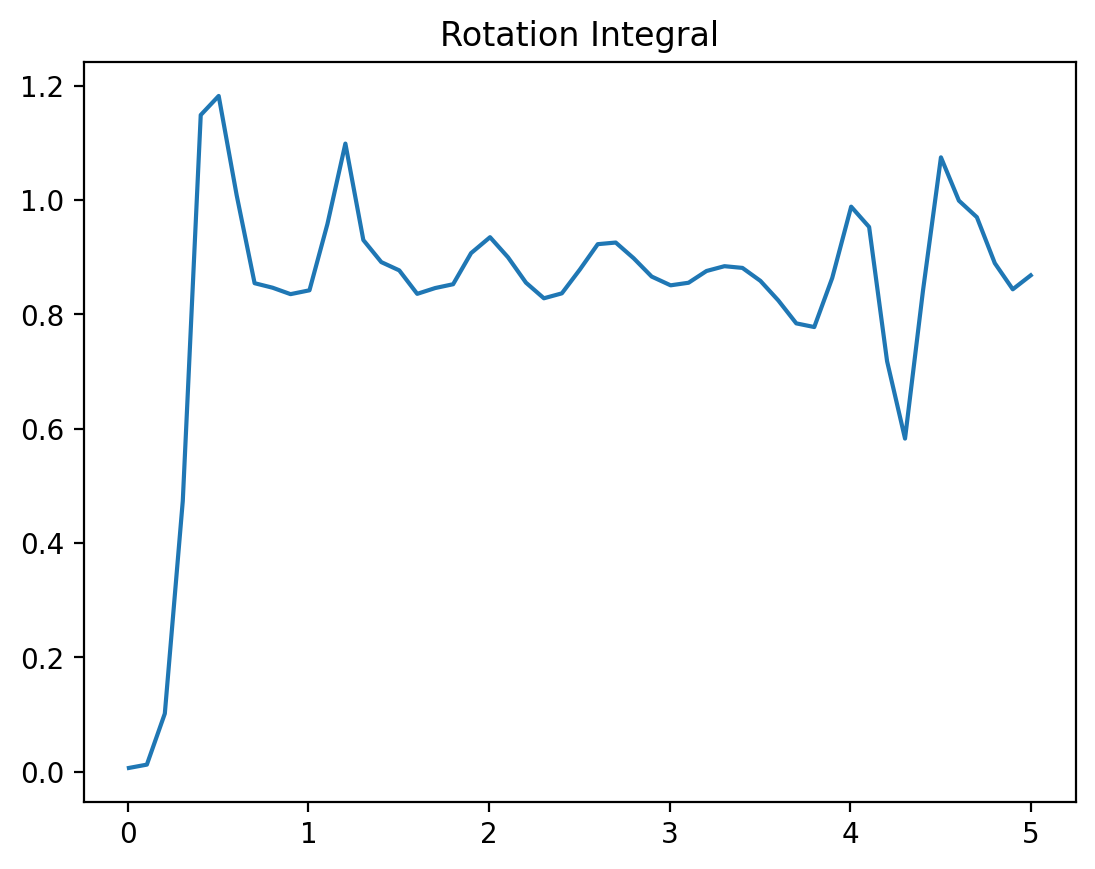
\includegraphics[width=0.87\textwidth]{imgs/results-KHI-RE10000.0-RSL128-rr_integral}
         \caption{resolution: 128}
         \label{fig:re10000-rs128}
     \end{subfigure}
        \caption{Magnitude of rotational part of the velocity gradient for varying grid resolutions}
        \label{fig:rr-resolution}
\end{figure}

I ran the simulation using different grid resolutions, all other parameter remained constant.
Figure \ref{fig:rr-resolution} depicts the magnitude of rotational part of the \ac{TDC} over time.

If found that meaningful rotations develop for a grid resolution of 32 or higher.
For a gird resolution of 16, the vortices never really manifested. Figure \ref{fig:re10000-rs16} supports this by showing that the rotational part of the \ac{TDC} remains (close to) zero. Figure \ref{fig:re16vs64} visualizes the vorticity field of the simulation at $t=4$ for resolutions 16 and 64.

We do not see noticeable differences in the instability onset between the other three simulations; however, grid resolutions 64 and 128 --- even though forming identical vortex structures in the beginning --- diverge already at t = 3. Figure \ref{fig:re128vs64} shows the diverged velocity fields.

\begin{figure}
     \centering
     \begin{subfigure}[b]{0.45\textwidth}
         \centering
         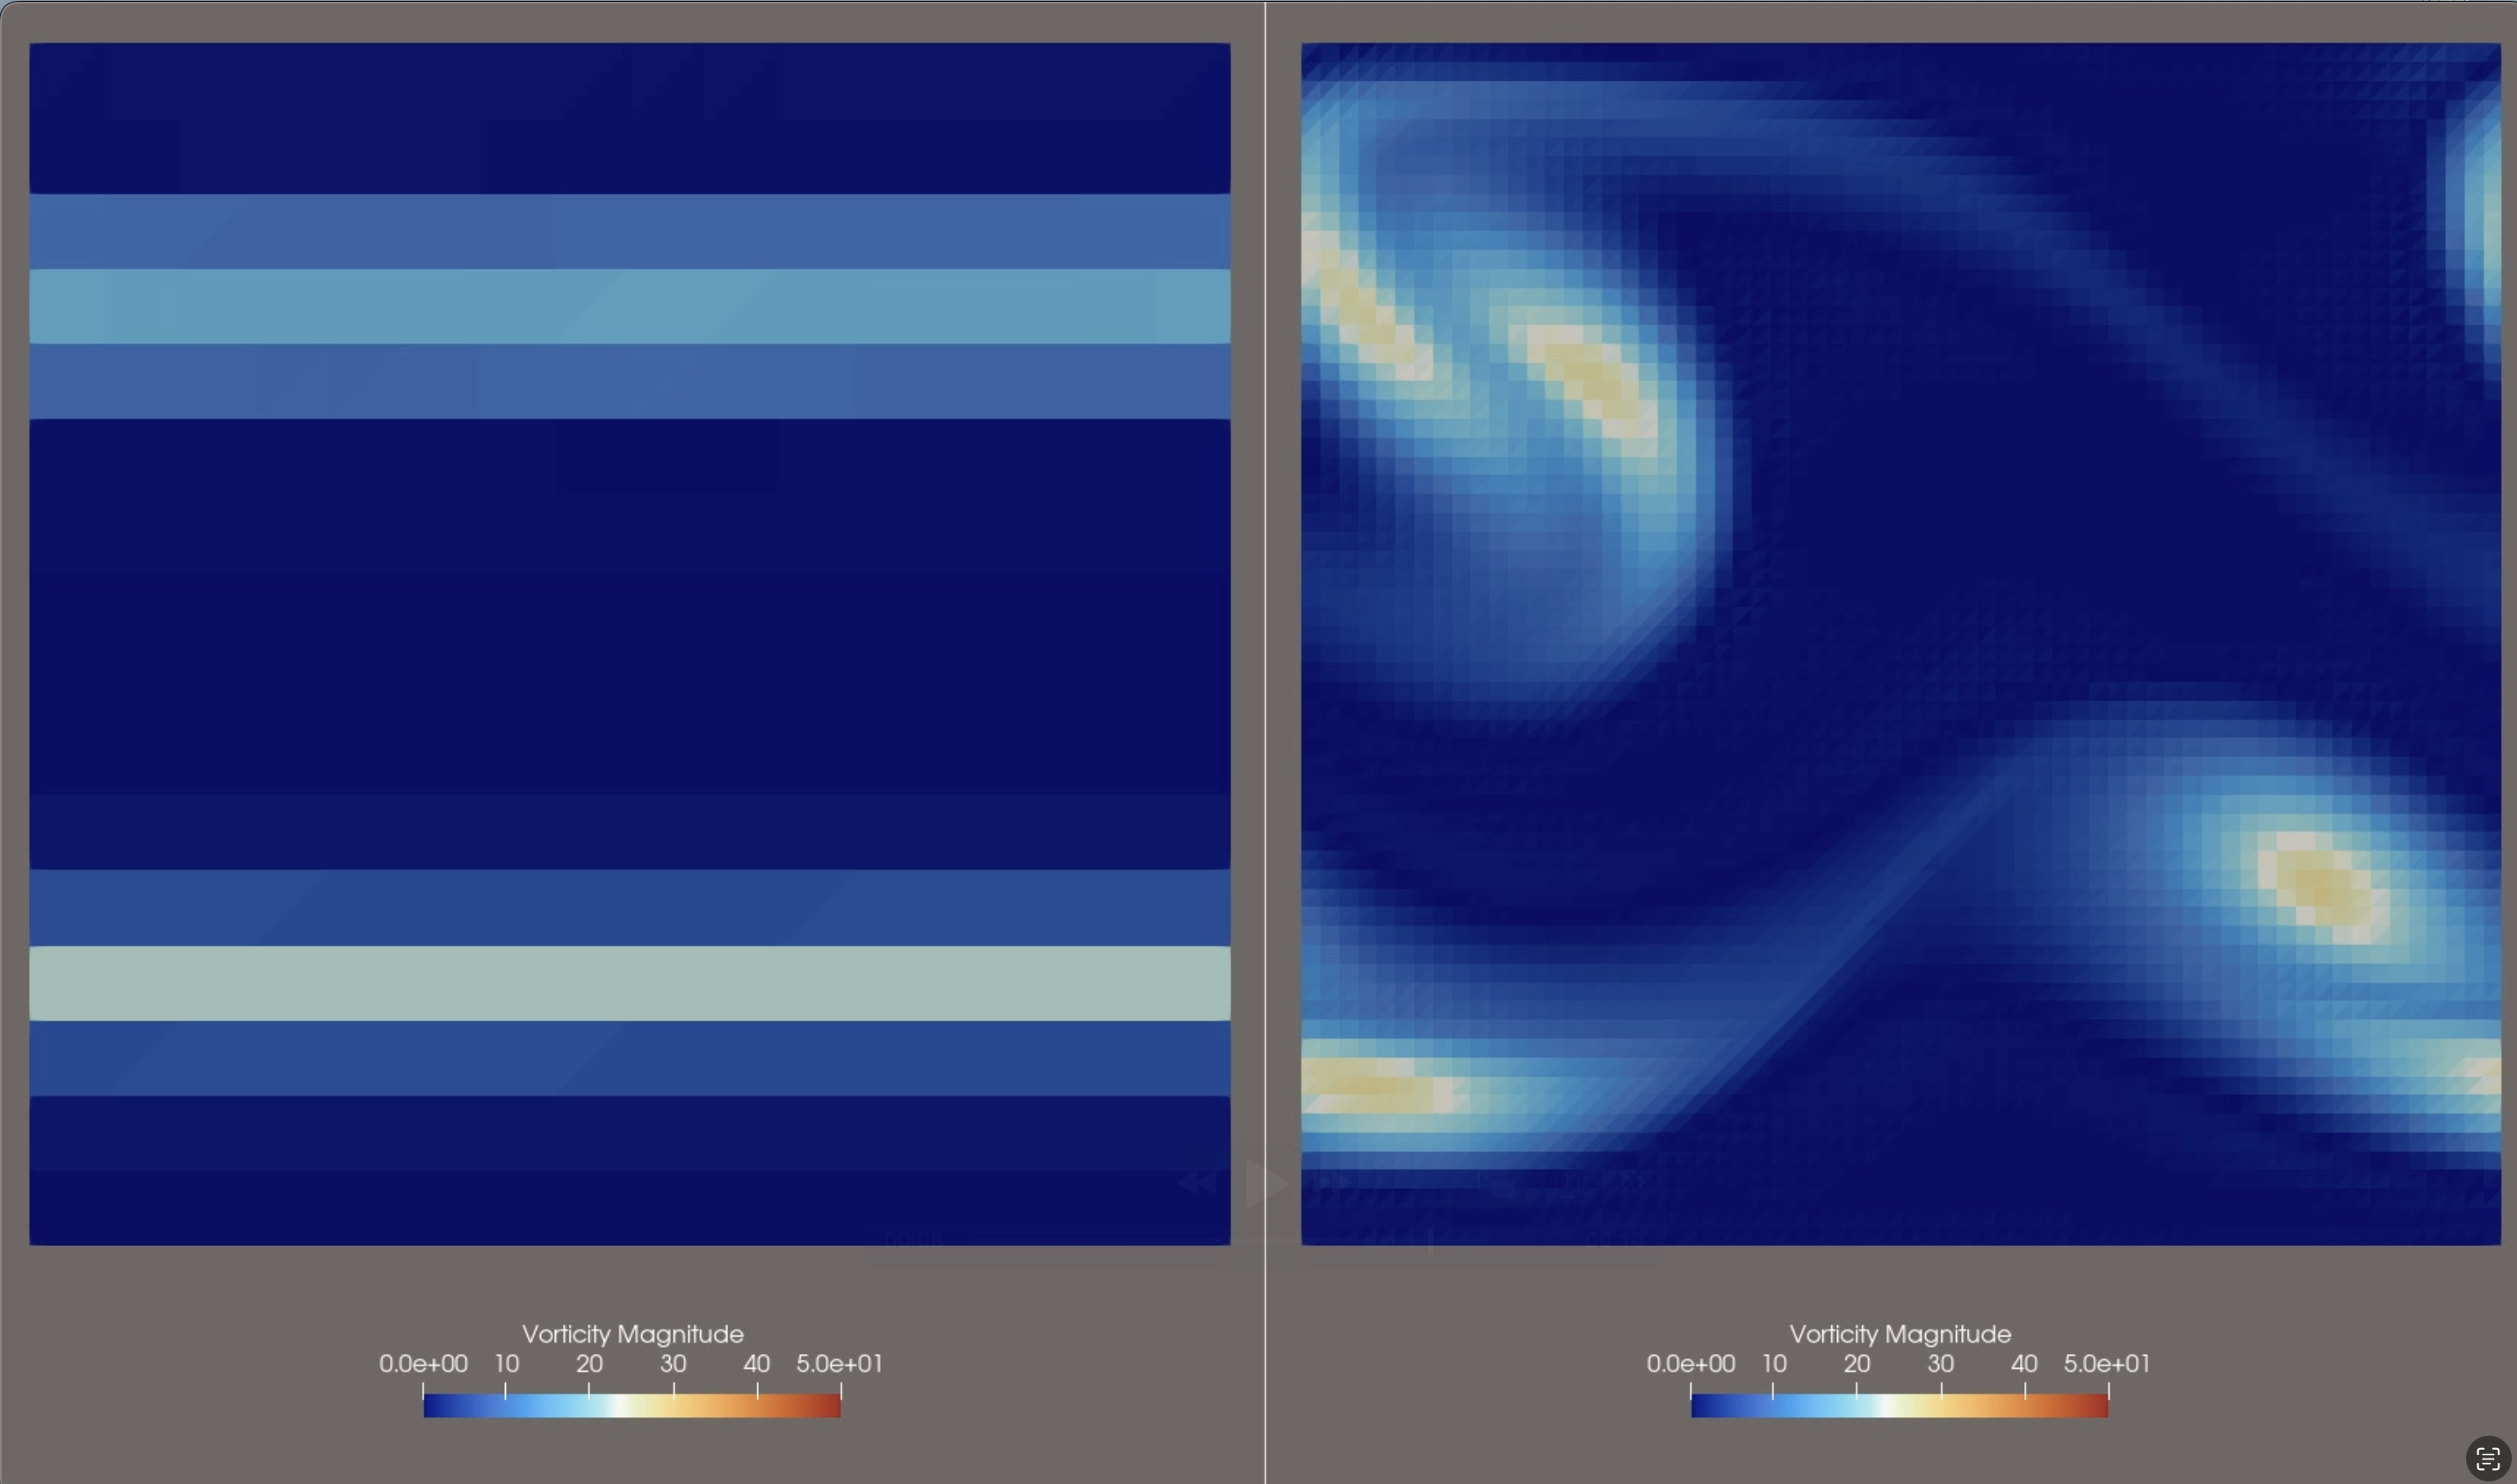
\includegraphics[width=\textwidth]{imgs/re16vs64}
         \caption{Resolution of 16 vs 64 at t=4}
         \label{fig:re16vs64}
     \end{subfigure}
     \hfill
     \begin{subfigure}[b]{0.45\textwidth}
         \centering
         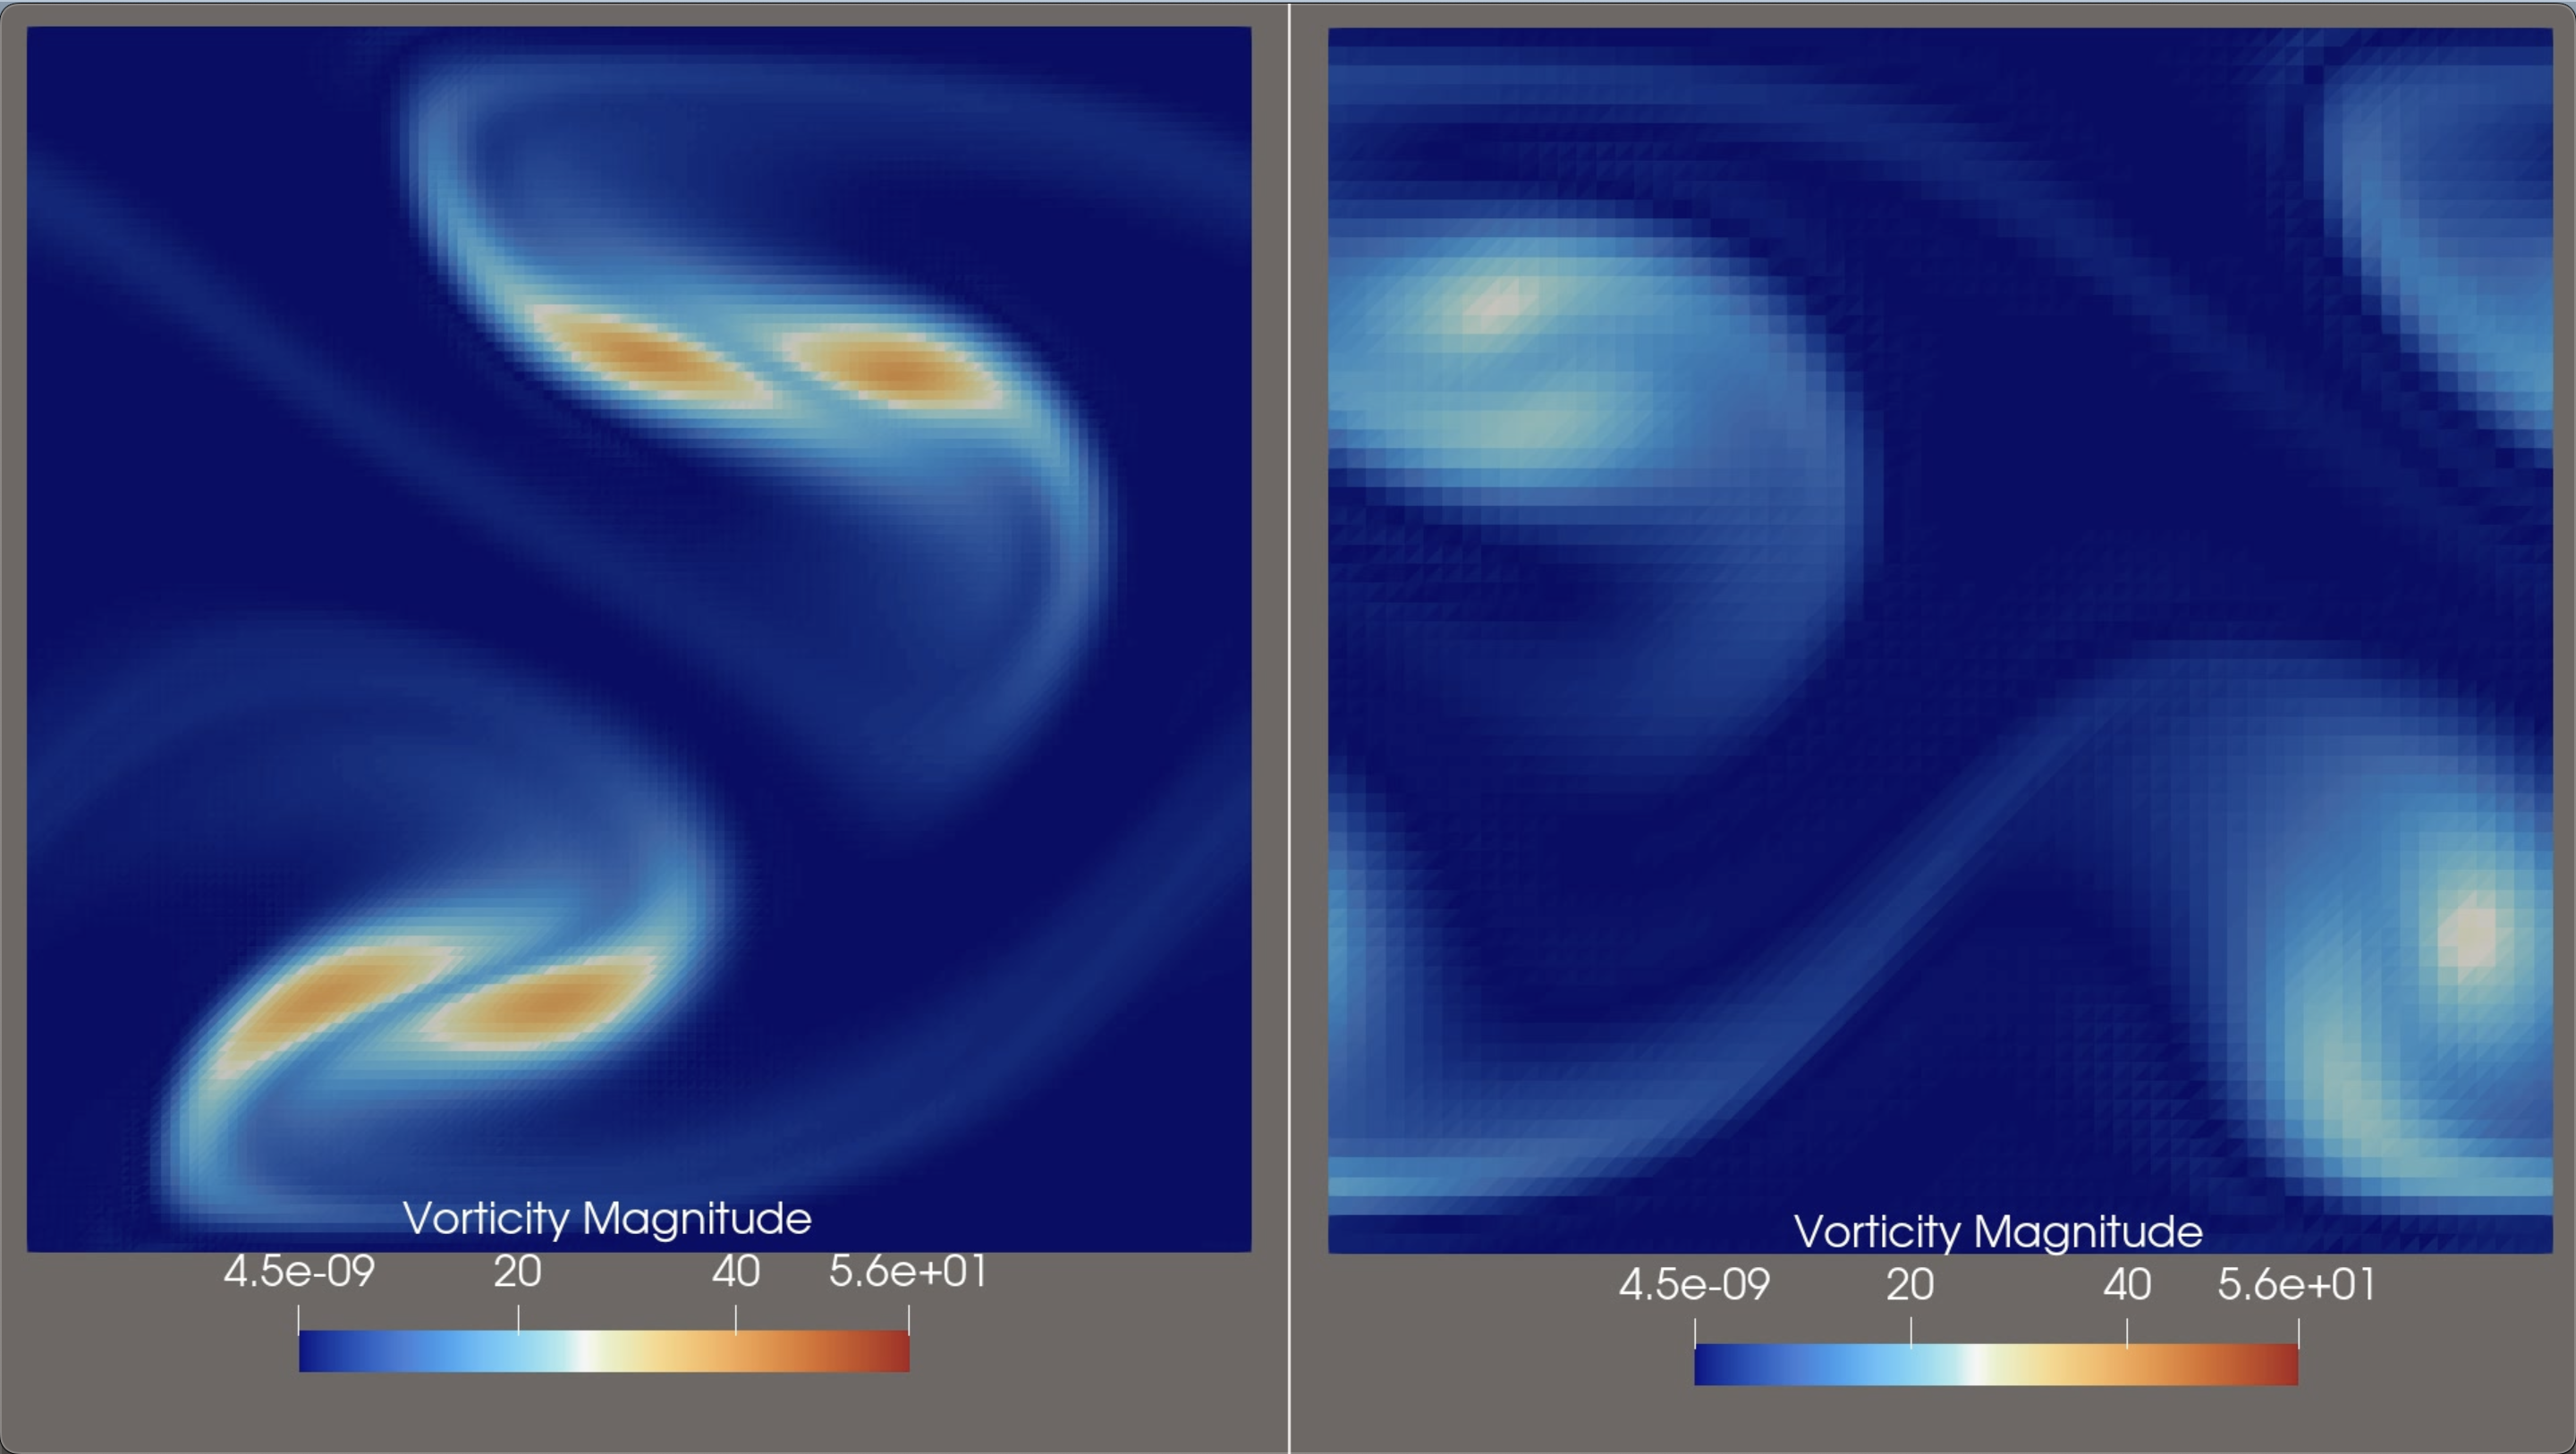
\includegraphics[width=\textwidth]{imgs/re128vs64}
         \caption{Resolution of 128 vs 64 at t=4}
         \label{fig:re128vs64}
     \end{subfigure}
     \caption{Curl: different resolutions in comparison.}
\end{figure}

\subsection{Dynamics for Different Reynolds Numbers}
\label{sec:result_reynolds}
\begin{figure}
     \centering
     \begin{subfigure}[b]{0.45\textwidth}
         \centering
         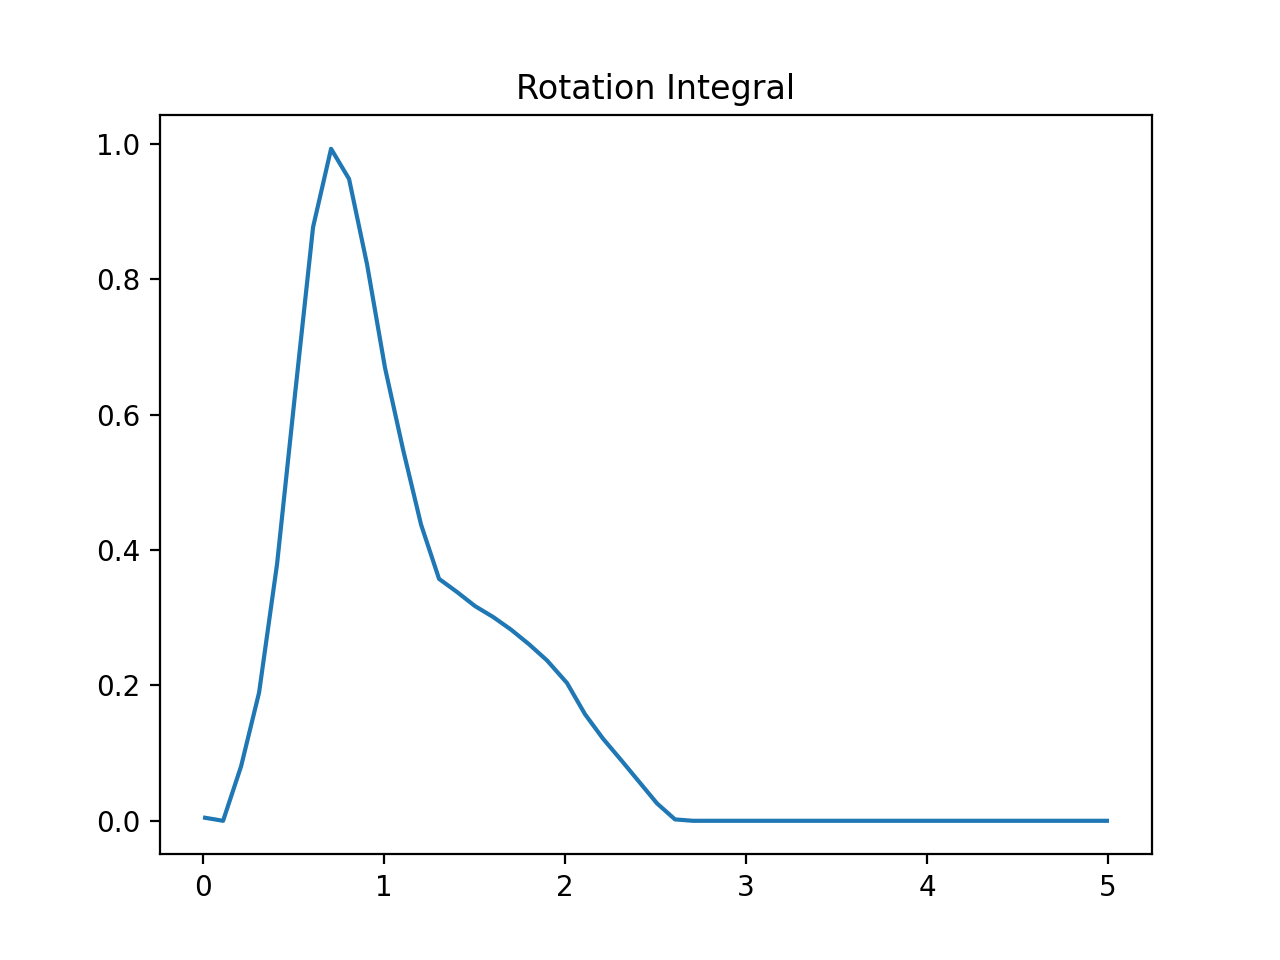
\includegraphics[width=\textwidth]{imgs/results-KHI-RE1000.0-RSL64-rr_integral}
         \caption{Reynolds number: 1e3}
         \label{fig:re1000-rs64}
     \end{subfigure}
     \hfill
     \begin{subfigure}[b]{0.45\textwidth}
         \centering
         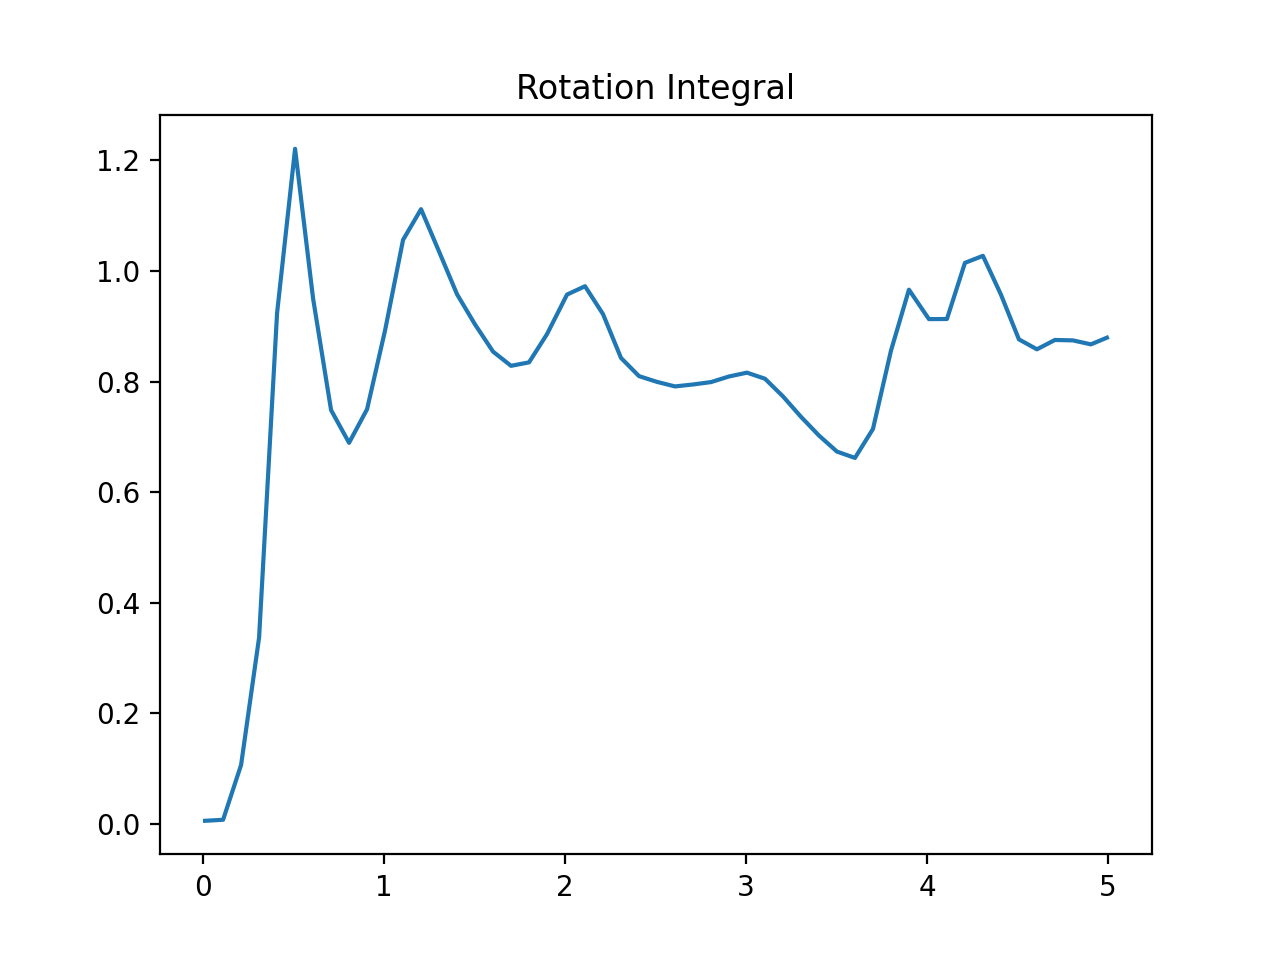
\includegraphics[width=\textwidth]{imgs/results-KHI-RE10000.0-RSL64-rr_integral}
         \caption{Reynolds number: 1e4}
         \label{fig:re10000-rs64-2}
     \end{subfigure}
     \hfill
     \begin{subfigure}[b]{0.45\textwidth}
         \centering
         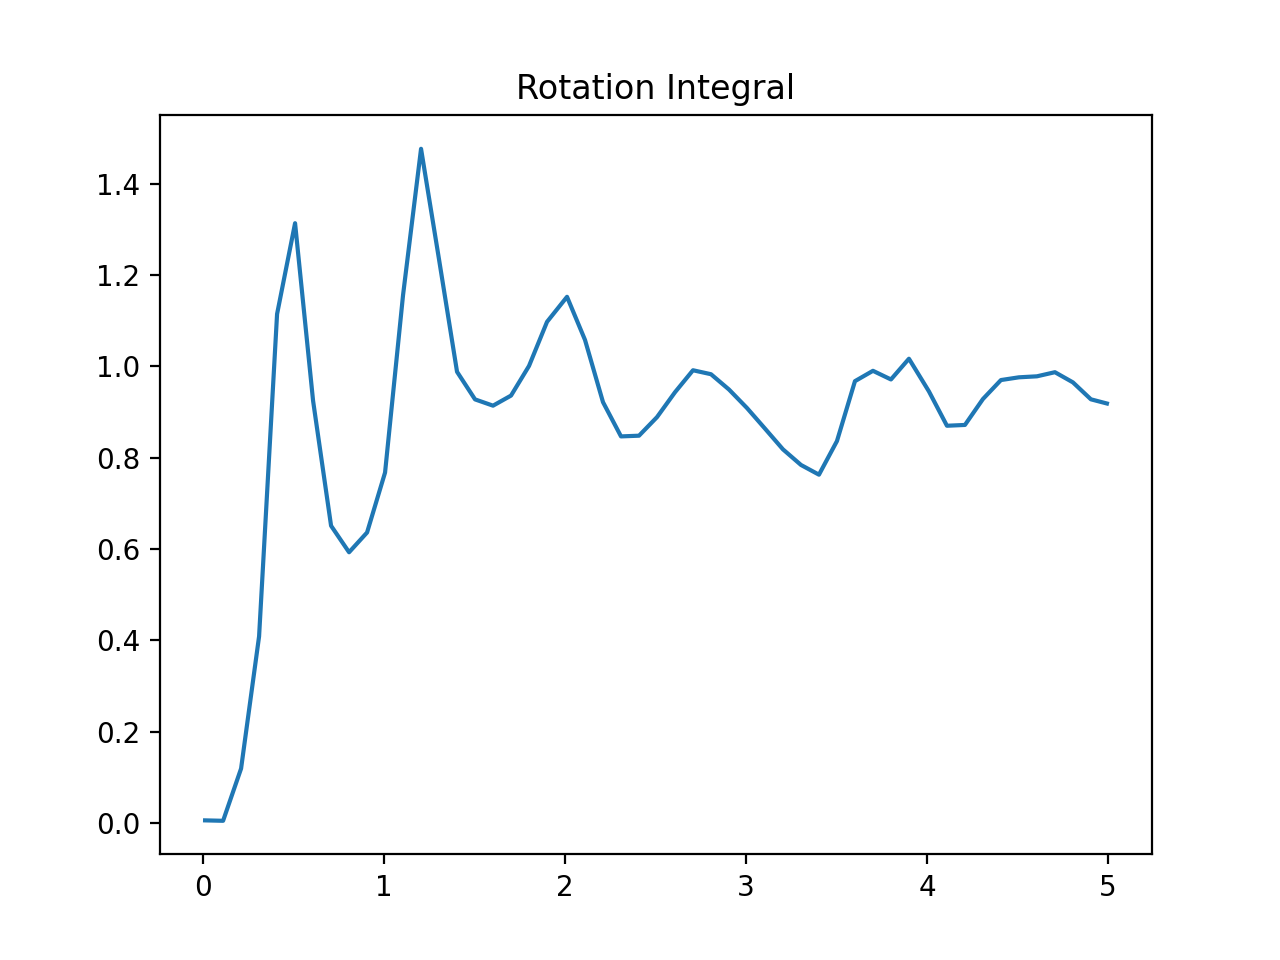
\includegraphics[width=\textwidth]{imgs/results-KHI-RE100000.0-RSL64-rr_integral}
         \caption{Reynolds number: 1e5}
         \label{fig:re100000-rs64}
     \end{subfigure}
     \hfill
     \begin{subfigure}[b]{0.45\textwidth}
         \centering
         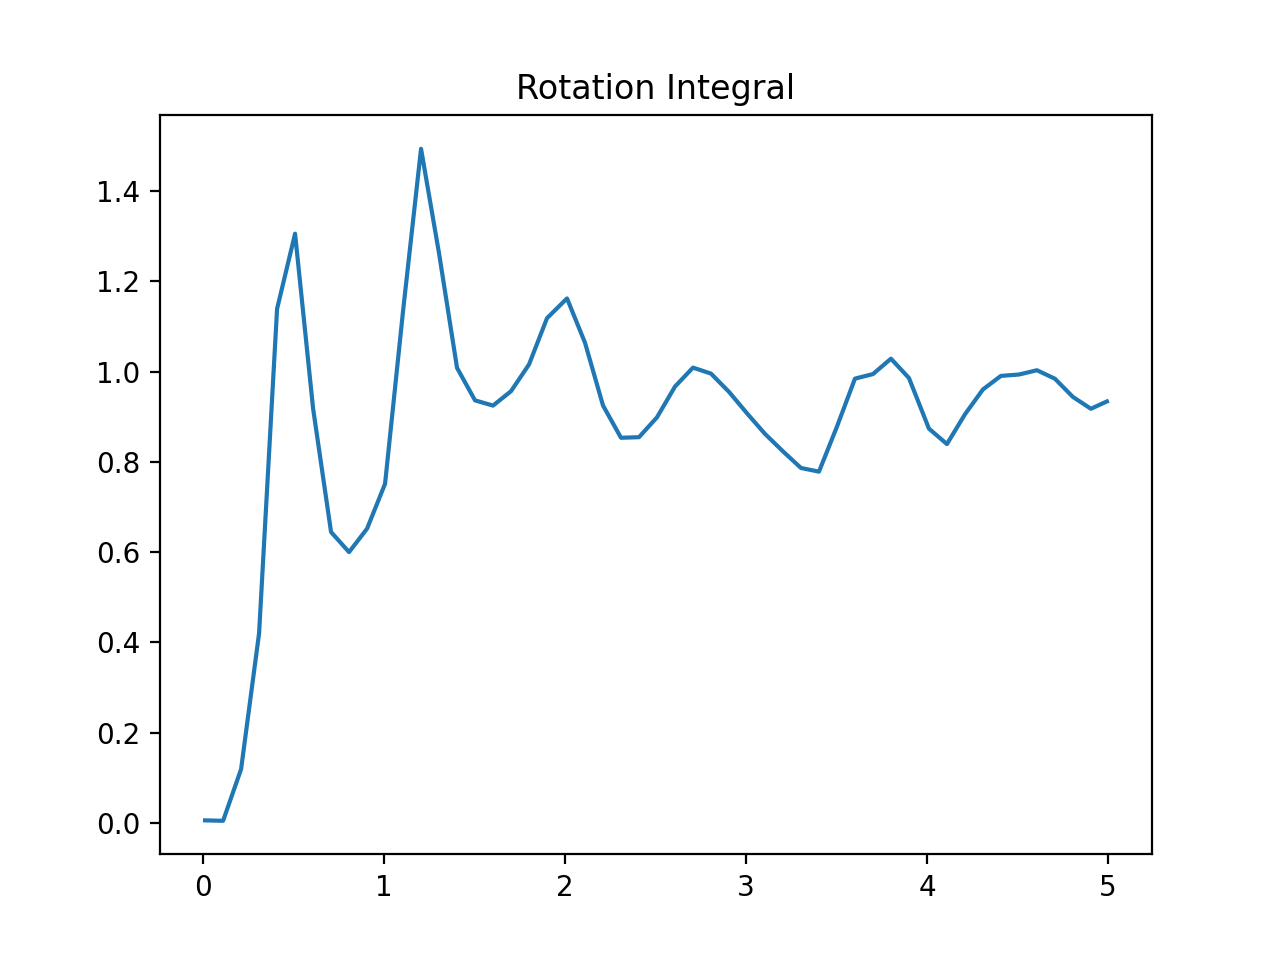
\includegraphics[width=\textwidth]{imgs/results-KHI-RE1000000.0-RSL64-rr_integral}
         \caption{Reynolds number: 1e6}
         \label{fig:re1000000-rs64}
     \end{subfigure}
     \caption{Magnitude of rotational part of the velocity gradient for varying Reynolds numbers}
     \label{fig:rr-reynoldnumber}
\end{figure}

I also ran the simulations for Reynold numbers 1e3, 1e4, 1e5 and 1e6, all with a resolution of 64 and same initial and boundary conditions.
As reference simulation I used the same simulation as in \ref{sec:result_grid}, meaning a Reynolds number of 1e4 and a grid resolution of 64.
For a Reynolds number of 1000, we see that the instability does initiates but then dissolves quickly.
The simulations with Reynolds numbers $1e4, ..., 1e6$ display persistent instabilities for the runtime of the simulation.
They share very similar behaviour and are nearly indistinguishable in the visualisation.
Only the magnitude of the rotations is slightly higher for Reynolds numbers $1e5$ and $1e6$ compared to the reference simulation.

\section{Discussion}
Simulating the \ac{K-H} instabilities was overall very successful.
I achieved in producing similar results in comparison to the example I used.
Behaviour differences were to be expected, mainly due to the use of different equations --- I used the incompressible Navier-Stokes equations, whereas the model used the Euler Fluid Equations for an optimal compressible gas).
Future work could change this to better replicate the model work.

\subsection{K-H Instabilities for different grid resolutions}
Simulating the \ac{K-H} instabilities over varying grid sizes demonstrated the need of a sufficiently resolved grid to guarantee representative solutions.
Firstly, the shear layer is not resolved correctly, leading to artificial diffusion and therefore in less shear force.
Secondly, under resolved grids lead to underestimating velocity gradients.
This is due to the smoothing introduced by the interpolation and discretisation process.
Lastly, the initial perturbation is smoothed as well for under resolved grids, making it harder for the instability to form.

For high enough grid resolutions the instability can remain stable over the simulation time as clearly visible in Figure \ref{fig:rr-resolution}.
The magnitude of the rotational part of the \ac{TDC} is also measurably higher, most likely due to the sharper velocity gradients.

\subsection{K-H Instabilities for different Reynolds numbers}
We saw in section \ref{sec:result_reynolds} that instabilities manifested even in the simulation with Reynolds number 1000.
It therefore is above the critical threshold.
However, the viscous dissipation is still very strong.
To my understanding, they act in a diffusing manner, forcing the vortices to smooth out.
This way, no secondary instabilities or vortices can develop.

For Reynolds numbers $1e4, 1e5$ and $1e6$, we can not see large differences in the simulation results.
It may be necessary to simulate longer time periods to see if the simulations diverge at a later point.
Future work could extend this, by simulating an even bigger range of fluids --- or use the Euler Fluid Equations as mentioned above.
I was not able to identify the critical threshold with this set of experiments, future work needs to extend the experiment to even lower Reynolds numbers.

\subsection{On the scientific method of this project}
To me this project was intended as a learning tool to get started in the world of \ac{CFD}.
For meaningful results, one should implement well known benchmark scenarios, e.g. \cite{Lehrenfeld2024}.
Without this verification the scientific value is very debatable.
The author realises this and wants to emphasise that he is still very satisfied with the learning outcomes of this project.

\section{Conclusion}
This project successfully demonstrates the sensitivity of Kelvin–Helmholtz instability simulations to both grid resolution and Reynolds number. Through implementation in FEniCS, it was shown that a minimum grid resolution is necessary to resolve shear layers and initiate the instability mechanism. Likewise, simulations with lower Reynolds numbers exhibited rapid dissipation of vortex structures, highlighting the diffusive role of viscosity in suppressing rotational dynamics. 
Conversely, for higher Reynolds numbers ($\geq 10^4$), vortices remained persistent, and the simulation outcomes became less sensitive to further increases in Reynolds number over the time period studied.

This work lacks validation against standardized benchmarks and is limited in scope. Still, it provided valuable insight to the author into the dynamics of shear-driven flows and the numerical requirements to capture them.
The results underscore the importance of both physical parameters and numerical resolution in \ac{CFD} simulations. For future work, validating against established test cases and extending the parameter range would strengthen the findings and further develop expertise in fluid instability modelling.

% content end
%###############################################################################
\newpage
\printbibliography

\section*{Appendix}
\begin{itemize}
    \item \href{https://colab.research.google.com/github/paulmyr/DD2365-AdvancedCFD/blob/master/project/template-report-Navier-Stokes.ipynb#scrollTo=W-bCOI6LuxFi}{Source Code}
    \item \href{https://github.com/paulmyr/DD2365-AdvancedCFD/tree/master/project/presentation/vid}{Simulation Renderings}
    \item \href{https://github.com/paulmyr/DD2365-AdvancedCFD/tree/master/project}{GitHub Repository}
    \item \href{https://www.deepl.com/de/translator}{DeepL: translations for the report.}
\end{itemize}

\end{document}